\chapter{Implementación de la aplicación}
\label{chap:appvalidation}

\section{Primera iteración}

\subsection{Alcance de la iteración}

En esta primera iteración se van a desarrollar los siguientes requisitos: RF1, RF2, RF3, RF4, RF5, RF6, RF7, RF8, RF9, RF12, RF13, RF14, RF15, RF16, RF17, RF18. 

Además, se deberá de crear la base de datos en Supabase, el proyecto en Flutter y conectarlos entre sí. Al final de la explicación de las iteraciones, se encuentra el diagrama de la base de datos junto a la explicación del proceso de creación de esta. 

Creando la aplicación en Flutter, se está asegurando el RNF2 - Compatibilidad. Flutter es una herramienta que permite programar en un lenguaje, Dart, y generar una aplicación compatible para cada sistema operativo (Android e IOS). 

Para la autenticación  (login / logout), se va a utilizar el sistema de autenticación de Supabase de correo electrónico y contraseña. Para evitar que cualquier persona pueda crearse una cuenta, las credeciales las proporcionará el desarrollador al usuario. Esto permite controlar el acceso al sistema y, con ello, mejorar la seguridad de la información. 

Además, Supabase dispone de "Auth policies" personalizables, lo que permite poner restricciones de acceso a la información de la base. Se pueden restringir ciertas operaciones y especificar aquellos roles que podrán hacer modificaciones en la base de datos. Esto permite proteger los datos almacenados en la base de datos, cumpliendo con el RNF1 - Seguridad. 

Para la gestión de clientes y artículos, se crearán las tablas convenientes. 

\subsection{Implementación}

La implementación se ha llevado a cabo en relación a los diseños de los bocetos iniciales del capítulo anterior. Además, se han añadido pantallas de categorías de artículos para permitir una mejor organización de los artículos de la tienda. Tras completar la implementación, hemos obtenido las siguientes pantallas: 

\subsubsection{Pantalla de login}

\begin{figure}[H]
	\centering
	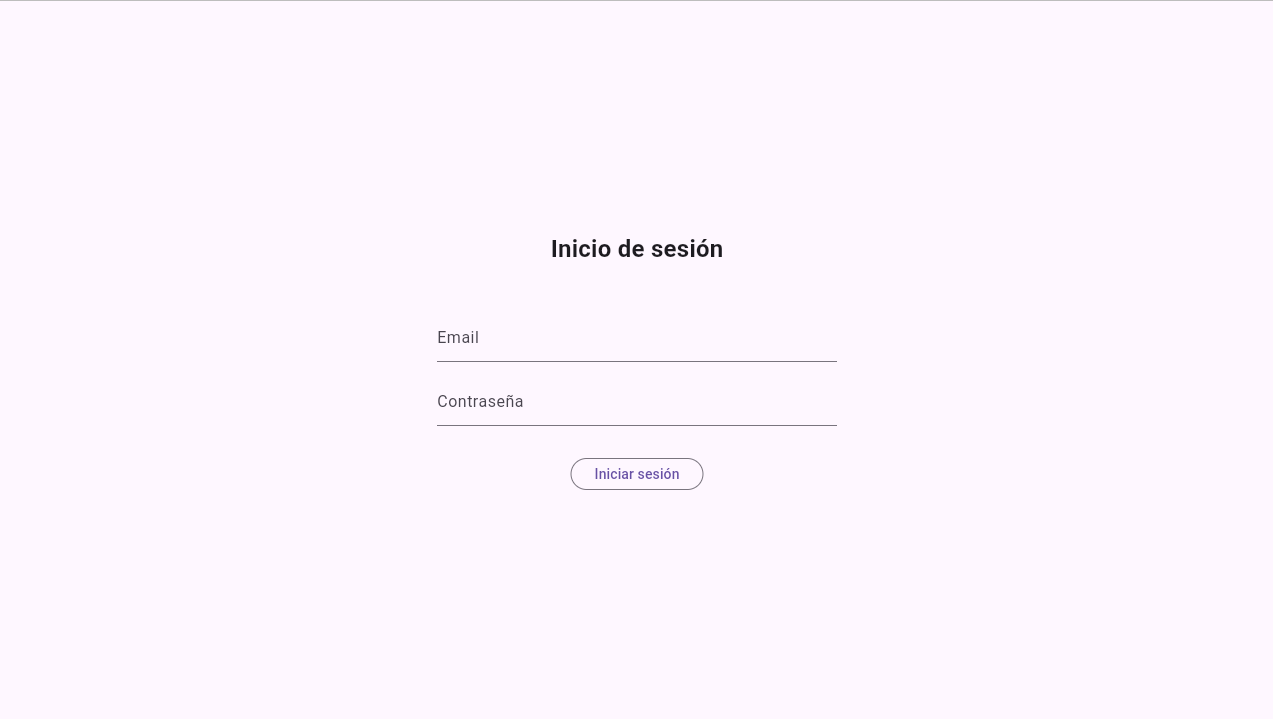
\includegraphics[width=0.7\textwidth]{imagenes/PrimeraIteracion/inicioSesion.png}
	\caption{Interfaz de usuario de inicio de sesión.}
	\label{fig:appInicioSesion}
\end{figure}

\subsubsection{Pantalla de principal}

\begin{figure}[H]
	\centering
	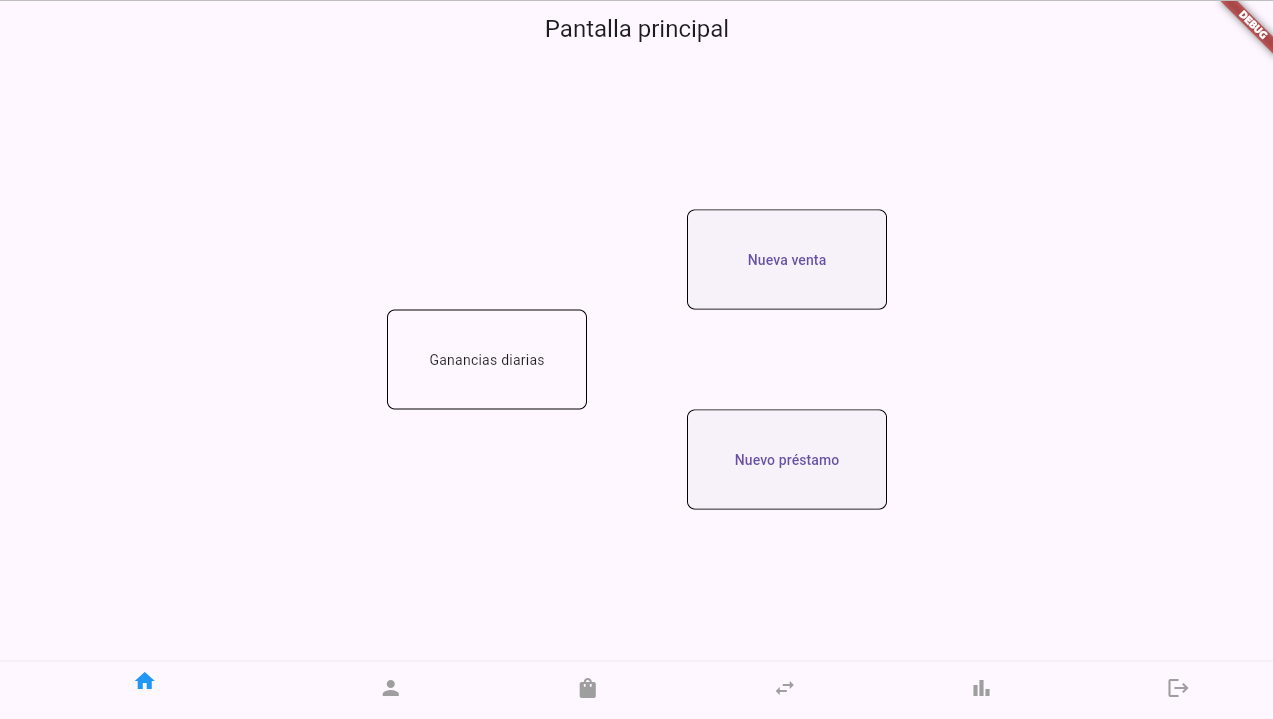
\includegraphics[width=0.7\textwidth]{imagenes/PrimeraIteracion/pantallaPrincipal.png}
	\caption{Interfaz de usuario de la pantalla principal.}
	\label{fig:appPantallaPrincipal}
\end{figure}

\subsubsection{Pantalla de visualización de clientes}

En esta pantalla se verán todos los clientes registrados en la tienda. Se pueden buscar por nombre o filtrar aquellos que deban dinero a la tienda. 

Los clientes que están en positivo en la tienda, es decir, tienen dinero a favor, se muestran con un fondo verde. Los clientes que están en negativo, se muestran con un fondo rojo. Si no tiene dinero a favor ni a deber, se muestran en blanco. 

\begin{figure}[H]
	\centering
	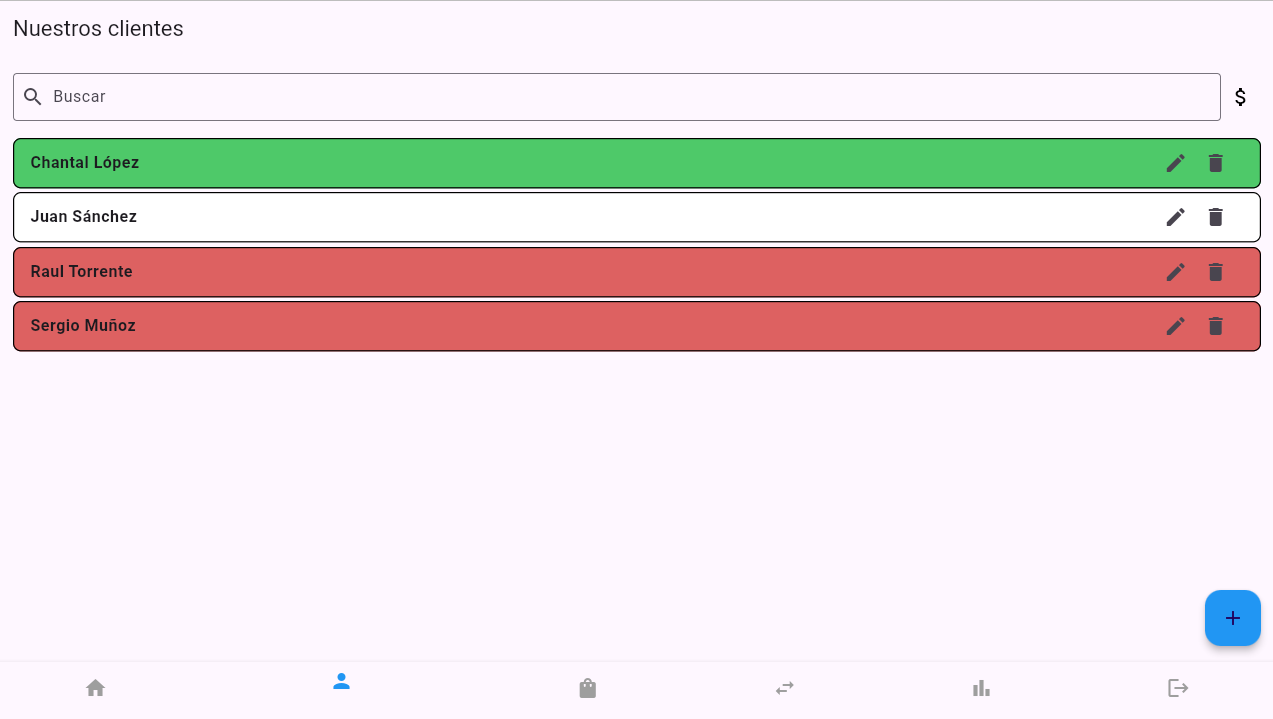
\includegraphics[width=0.7\textwidth]{imagenes/PrimeraIteracion/visualizacionClientes.png}
	\caption{Interfaz de usuario de la pantalla de visualización de clientes.}
	\label{fig:appVisualizarClientes}
\end{figure}

\subsubsection{Pantalla de añadir nuevo cliente}

\begin{figure}[H]
	\centering
	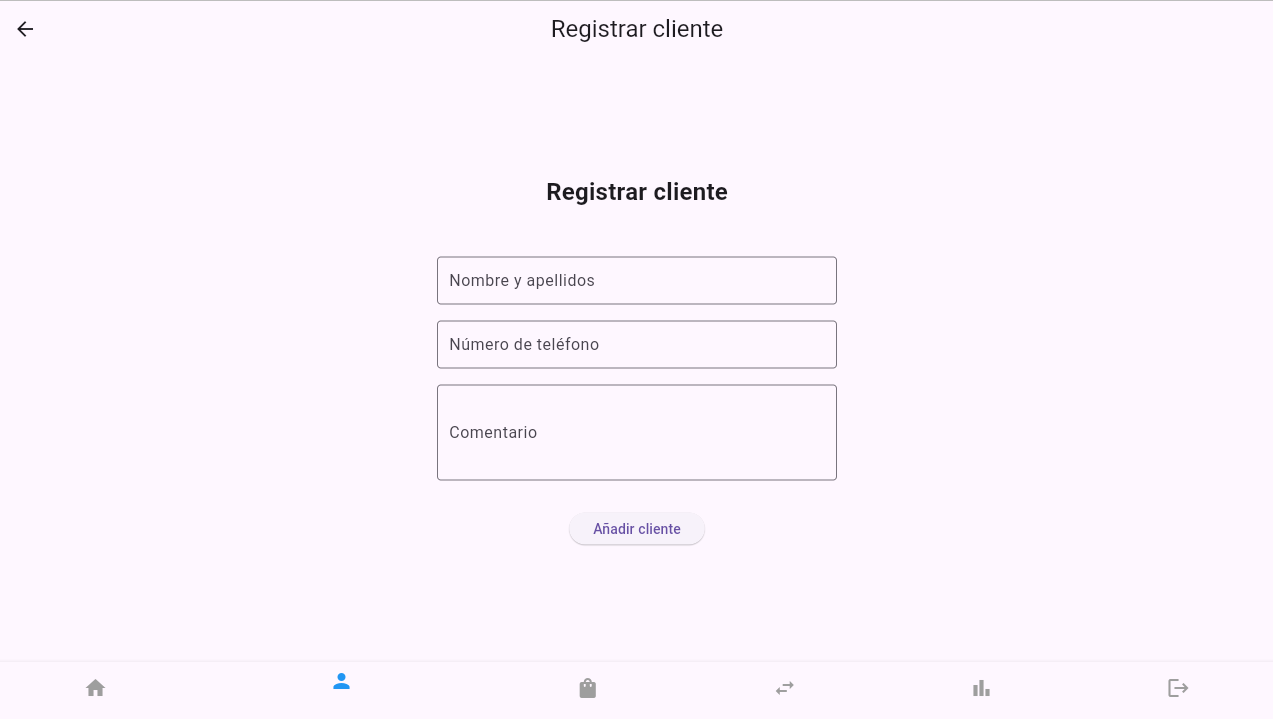
\includegraphics[width=0.7\textwidth]{imagenes/PrimeraIteracion/nuevoCliente.png}
	\caption{Interfaz de usuario de la pantalla de nuevo cliente.}
	\label{fig:appNuevoCliente}
\end{figure}

\subsubsection{Pantalla de editar un cliente existente}

\begin{figure}[H]
	\centering
	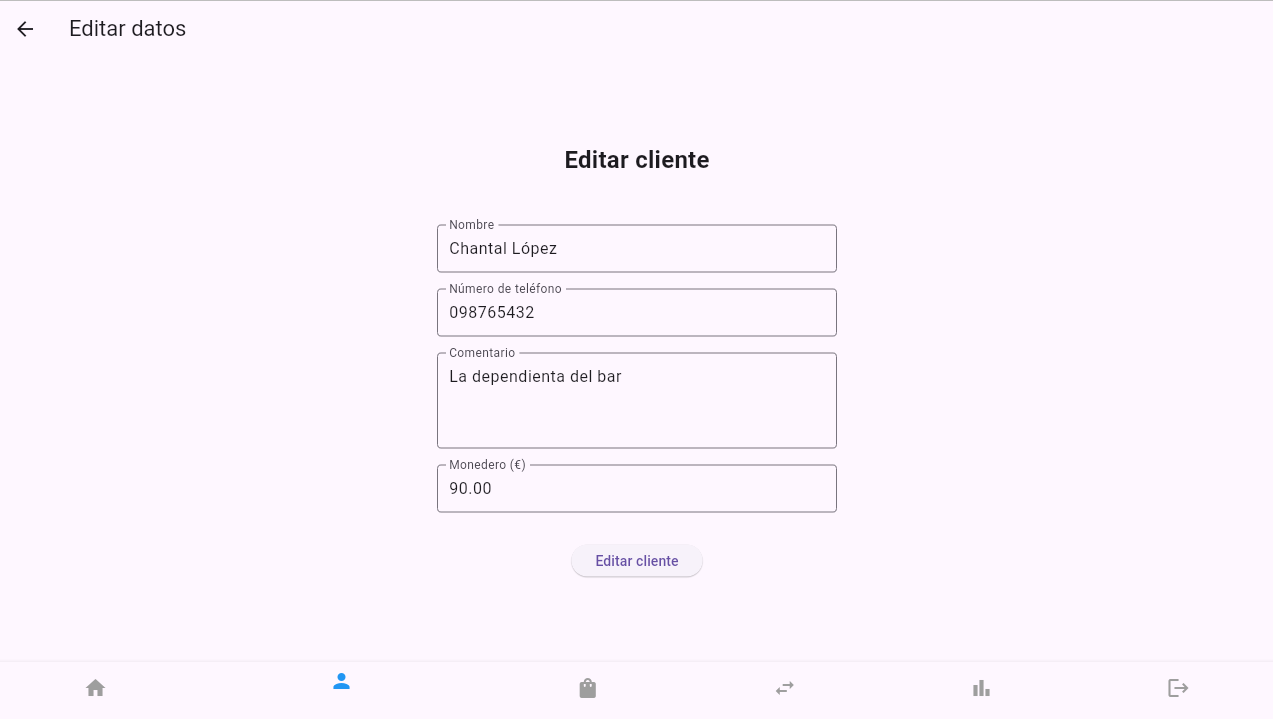
\includegraphics[width=0.7\textwidth]{imagenes/PrimeraIteracion/editarCliente.png}
	\caption{Interfaz de usuario de la pantalla de editar cliente.}
	\label{fig:appEditarCliente}
\end{figure}

\subsubsection{Pantalla de visualizar los datos de un cliente}

\begin{figure}[H]
	\centering
	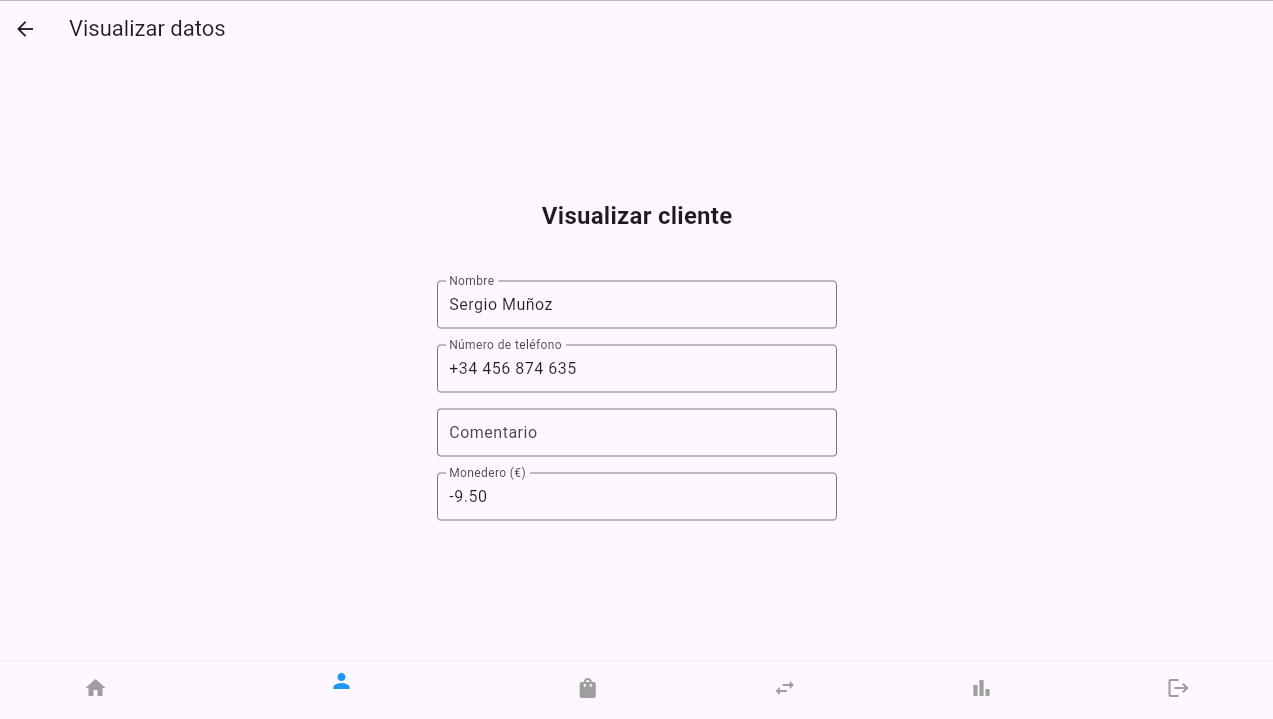
\includegraphics[width=0.7\textwidth]{imagenes/PrimeraIteracion/detallesCliente.png}
	\caption{Interfaz de usuario de la pantalla de visualizar datos de un cliente.}
	\label{fig:appDetallesCliente}
\end{figure}

\subsubsection{Pantalla de visualizar las categorías de artículos}

Se pueden añadir tantas categorías como el usuario crea conveniente para poder organizar los productos de su tienda a su gusto. 

\begin{figure}[H]
	\centering
	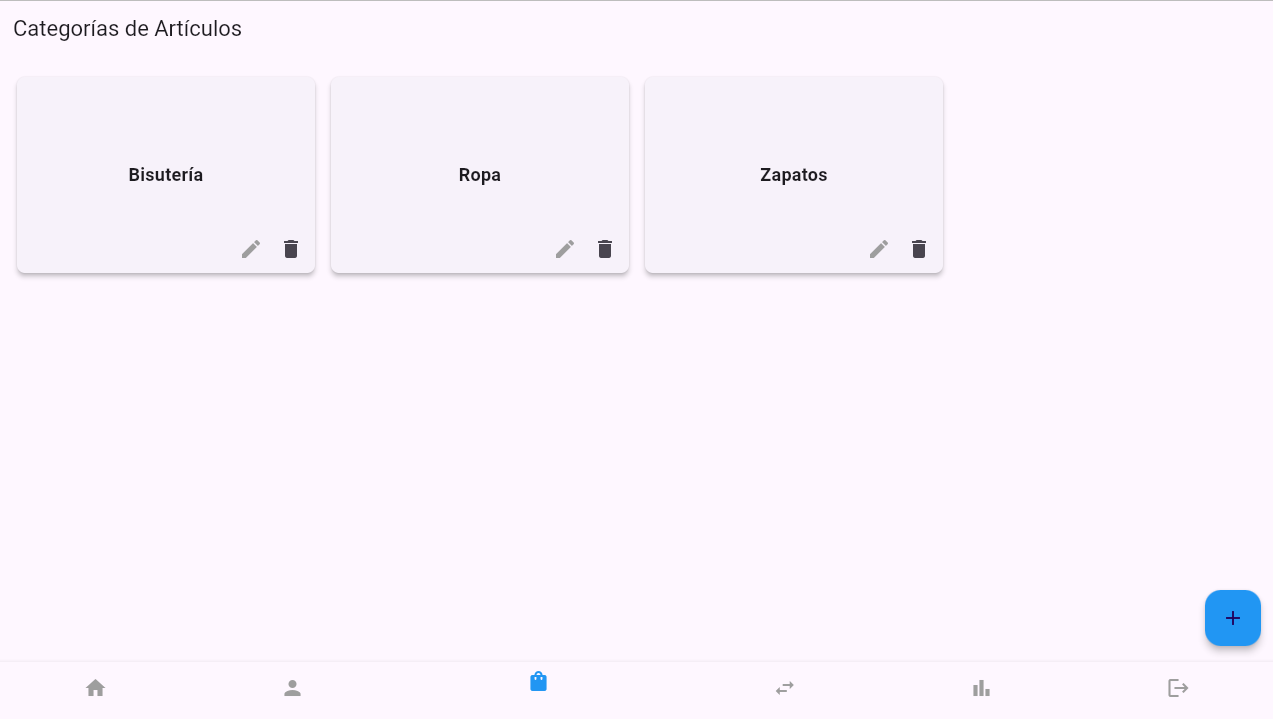
\includegraphics[width=0.7\textwidth]{imagenes/PrimeraIteracion/visualizarCategorias.png}
	\caption{Interfaz de usuario de la pantalla de visualizar las categorías.}
	\label{fig:appCategoriasArticulos}
\end{figure}

\subsubsection{Pantalla de añadir una nueva categoría de artículos}

Cuando se añade una nueva categoría, se deberá de especificar el nombre de dicha categoría y se podrán desmarcar los campos que no sean necesarios para esa categoría. Al marcar o desmarcar un campo, se cambia la visibilidad de este en todos los artículos que estén contenidos en esa categoría. Así se evita incluir campos que no tengan relevancia en ciertas categorías. 

\begin{figure}[H]
	\centering
	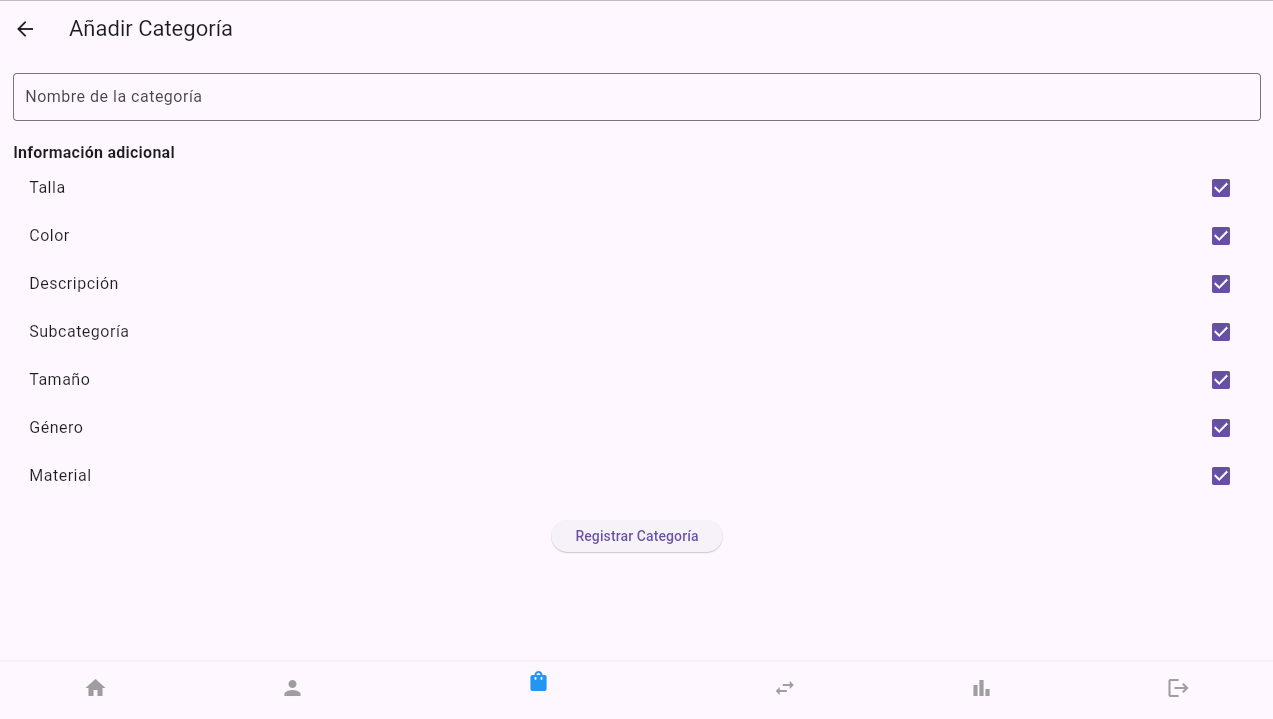
\includegraphics[width=0.7\textwidth]{imagenes/PrimeraIteracion/nuevaCategoria.png}
	\caption{Interfaz de usuario de la pantalla de añadir nueva categoría.}
	\label{fig:appNuevaCategoria}
\end{figure}

\subsubsection{Pantalla de editar una categoría existente}

\begin{figure}[H]
	\centering
	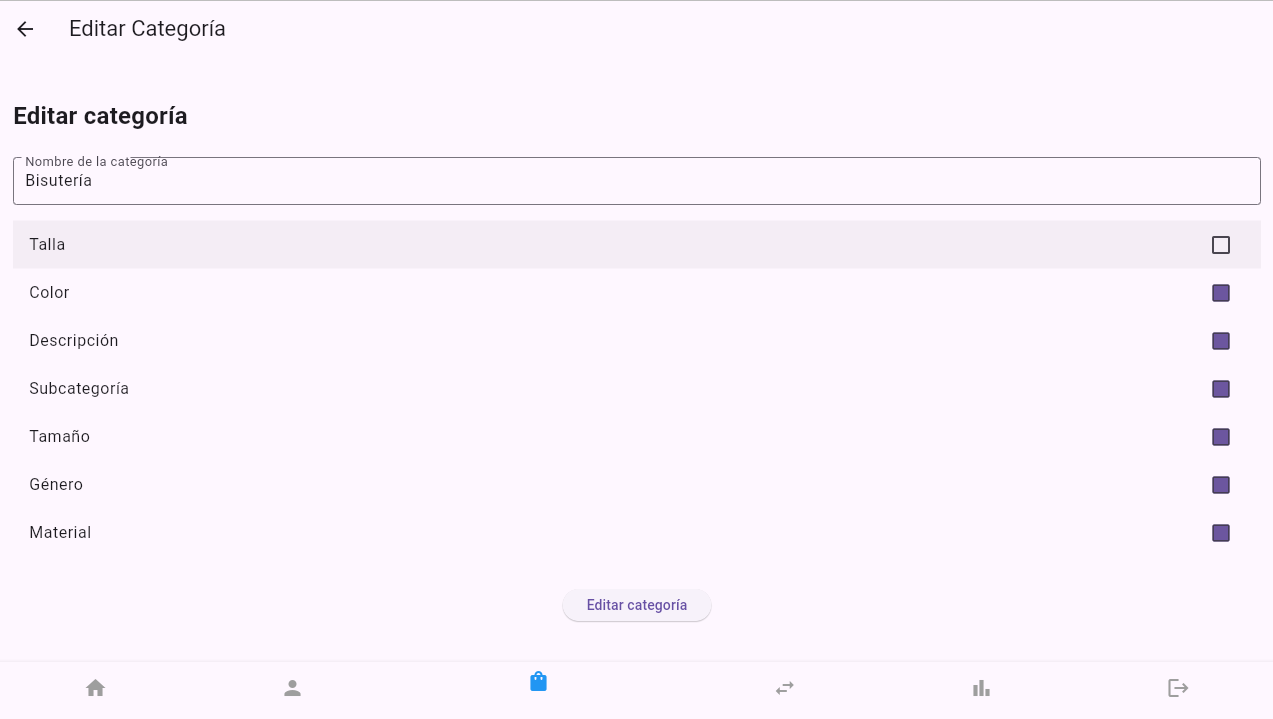
\includegraphics[width=0.7\textwidth]{imagenes/PrimeraIteracion/editarCategoria.png}
	\caption{Interfaz de usuario de la pantalla de editar una categoría.}
	\label{fig:appEditarCategoria}
\end{figure}

\subsubsection{Pantalla de visualizar los artículos de una categoría}

En esta pantalla se ven todos los artículos de una determinada categoría. Se puede buscar por nombre o filtrar por subcategoría. 

\begin{figure}[H]
	\centering
	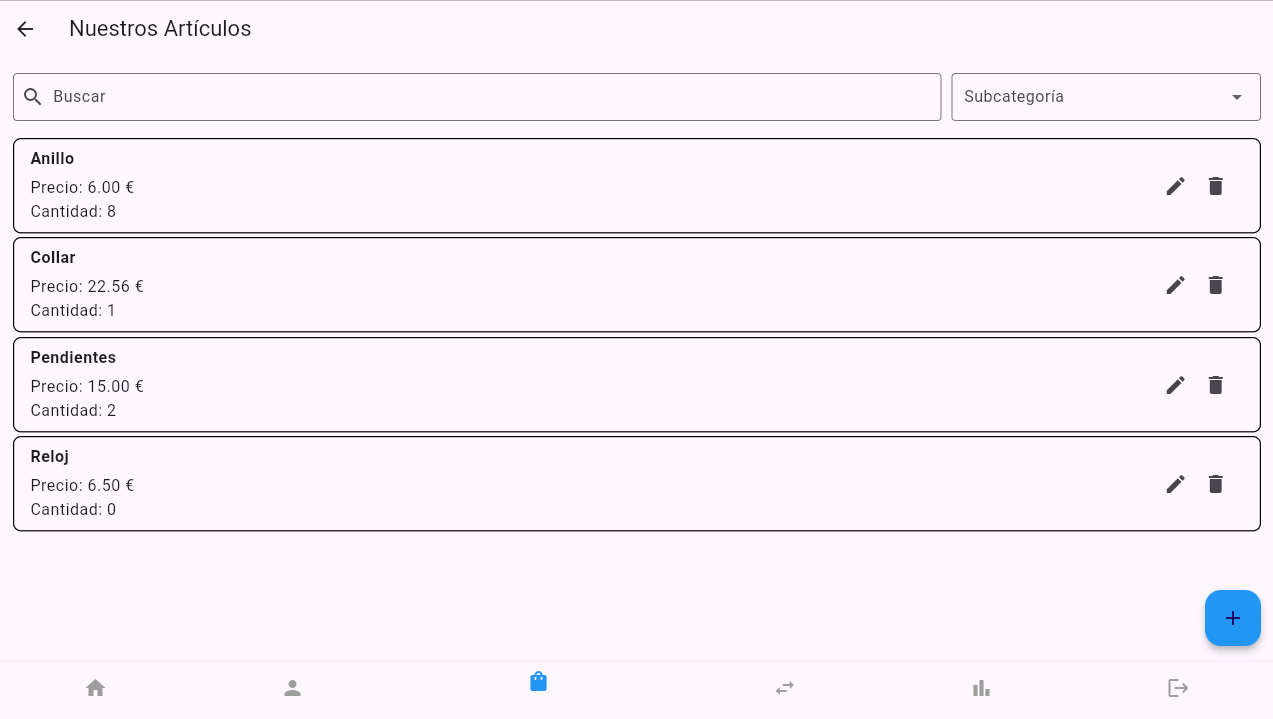
\includegraphics[width=0.7\textwidth]{imagenes/PrimeraIteracion/visualizarArticulos.png}
	\caption{Interfaz de usuario de la pantalla de visualizar artículos.}
	\label{fig:appVisualizarArticulos}
\end{figure}

\subsubsection{Pantalla de añadir un nuevo artículo a una categoría}

\begin{figure}[H]
	\centering
	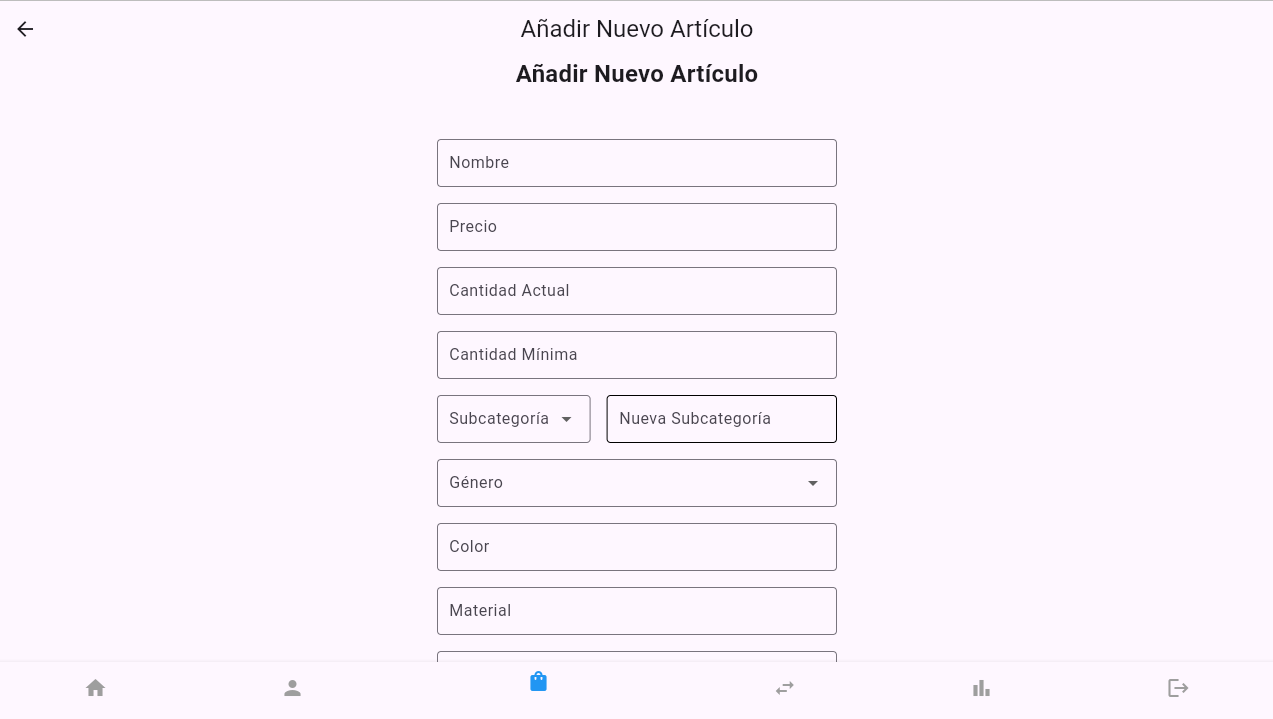
\includegraphics[width=0.7\textwidth]{imagenes/PrimeraIteracion/nuevoArticulo.png}
	\caption{Interfaz de usuario de la pantalla de añadir un nuevo artículo.}
	\label{fig:appNuevoArticulo}
\end{figure}

\subsubsection{Pantalla de editar un artículo existente de una categoría}

\begin{figure}[H]
	\centering
	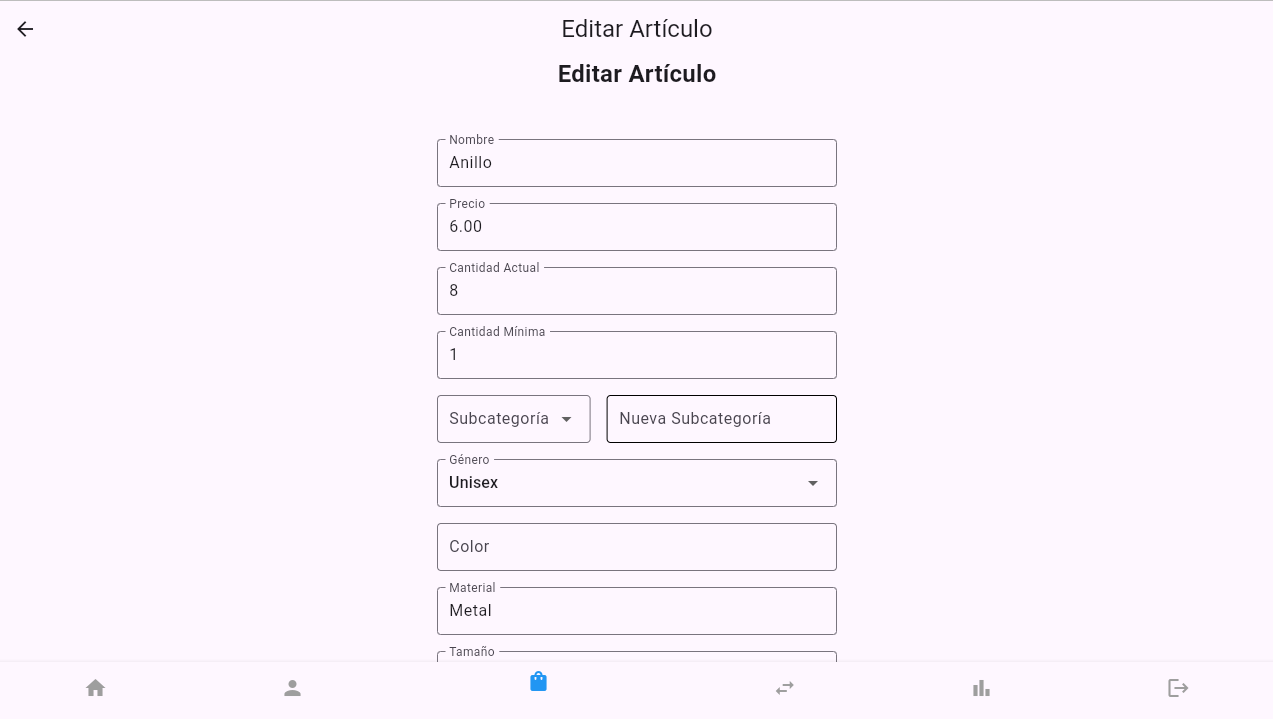
\includegraphics[width=0.7\textwidth]{imagenes/PrimeraIteracion/editarArticulo.png}
	\caption{Interfaz de usuario de la pantalla de editar un artículo existente.}
	\label{fig:appEditarArticulo}
\end{figure}


\subsection{Revisión de la iteración}

\subsubsection{Autenticacion}

El cliente probó el sistema de autenticación y le pareció correcto. 

\subsubsection{Gestión de clientes}

El cliente probó este conjunto de pantallas que gestionan los clientes de la tienda. Pidió una mejora en la accesibilidad en la pantalla de visualizado de clientes. No diferenciar únicamente cuando un cliente debe con un sistema de colores (verde/rojo), añadir también un icono que lo represente. El resto de funcionalidades estaban correctas. 

\subsubsection{Gestión de artículos}

El cliente probó este conjunto de pantallas que gestionan los artículos de la tienda y decidió que no se estaban organizando de forma correcta. Las categorías estaban bien, pero a la hora de añadir nuevos artículos, el formulario debería de permitir añadir varias tallas, no únicamente una. Además, por cada talla, se debería de gestionar la cantidad actual, cantidad mínima y color. 

El resto de funcionalidades estaban bien.  


\subsection{Plan para la próxima iteración}

Para la próxima iteración se propone:

\begin{itemize}
	\item Implementar las mejoras señaladas por el cliente.
	\item Implementar la pantalla de la lista de renovación de artículos.
	\item Implementar las pantallas de gestión de movimientos.
\end{itemize}

\newpage

\section{Segunda iteración}

\subsection{Alcance de la iteración}

En esta segunda iteración se van a desarrollar los siguientes requisitos: RF10, RF19, RF20, RF21, RF22, RF23, RF24, RF25, RF26, RF27, RF28. 

Además se han mejorado los siguientes requisitos como consecuencia de las mejoras señaladas por el cliente: RF3, RF4, RF6.

\subsection{Implementación}

La implementación se ha llevado a cabo en relación a los diseños de los bocetos iniciales del capítulo anterior. Estos bocetos eran orientativos y el diseño se ha mejorado en esta etapa para obtener una mejor usabilidad. Tras completar la implementación, hemos obtenido las siguientes pantallas: 

\subsubsection{Pantalla principal}

En esta pantalla se pueden consultar las ganancias diarias y se muestran las opciones de generar una nueva venta o un nuevo préstamo. Esto se ha puesto en la pantalla principal ya que son las funcionalidades que se usarán con más frecuencia. 

\begin{figure}[H]
	\centering
	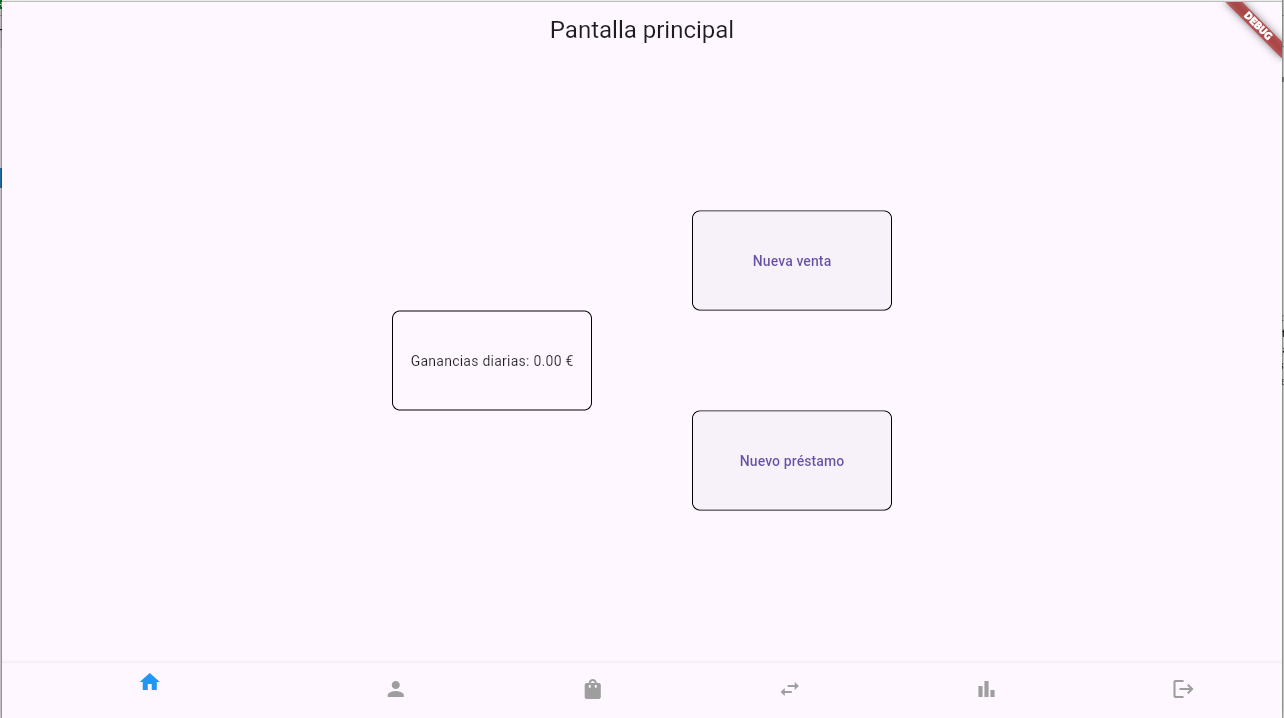
\includegraphics[width=0.7\textwidth]{imagenes/SegundaIteracion/pantallaPrincipal.png}
	\caption{Interfaz de usuario de la pantalla principal.}
	\label{fig:appPantallaPrincipal}
\end{figure}

\subsubsection{Pantalla de nueva venta}

En esta pantalla se realiza una nueva venta. En el buscador de la parte superior, se van proponiendo artículos que coincidan con los caracteres buscados. Una vez seleccionado el artículo, en los desplegables de la talla y el color, se proponen únicamente las tallas o colores que existan para dicho artículo. La cantidad no puede ser inferior a 1. Si la cantidad es mayor a la que hay disponible en la tienda, salta un error avisando de que la cantidad es errónea. Si todo es correcto, pulsando al + se añade el artículo a la lista. Como es una venta, asignar el cliente es opcional. También es una búsqueda dinámica como el buscador de los artículos. El método de pago es obligatorio y se podrá elegir entre Efectivo y Tarjeta. Una vez todos los campos estén completos y se pulse al botón de Aceptar, se generará un nuevo movimiento tipo Venta.

\begin{figure}[H]
	\centering
	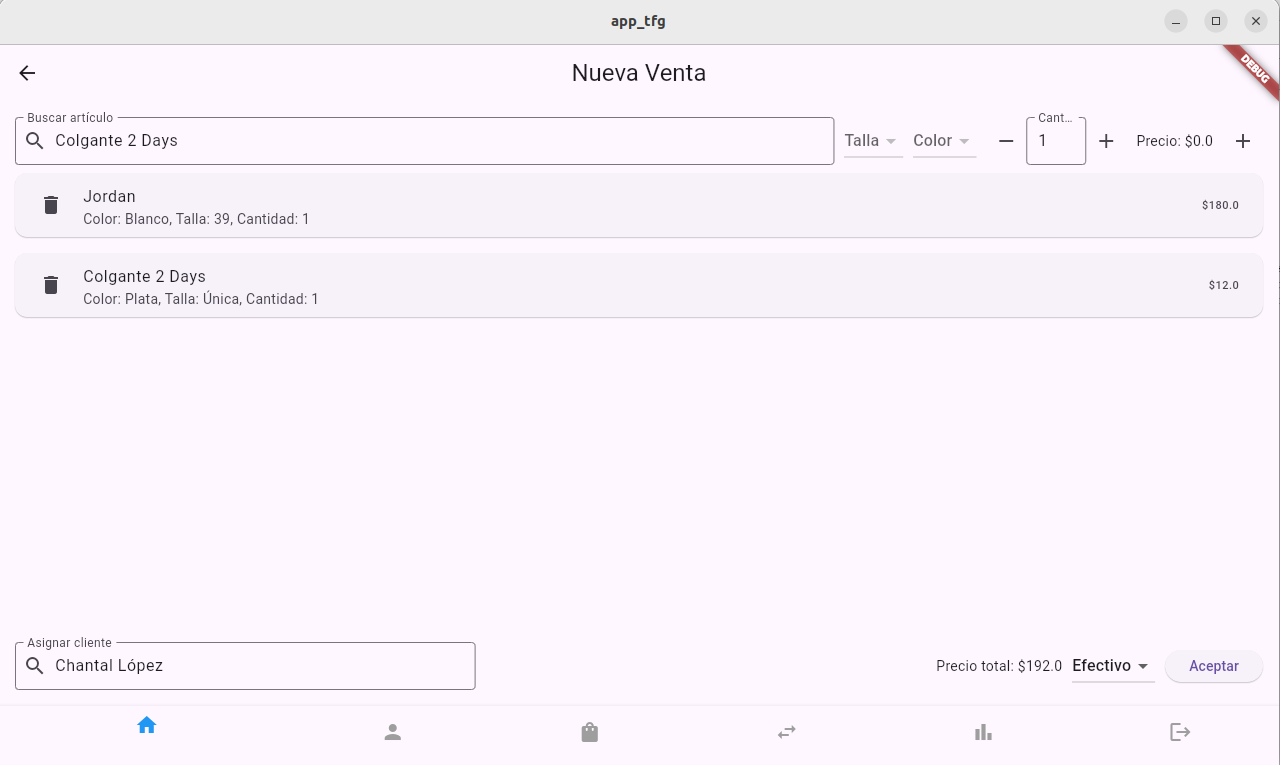
\includegraphics[width=0.7\textwidth]{imagenes/SegundaIteracion/nuevaVenta.png}
	\caption{Interfaz de usuario de la pantalla de nueva venta.}
	\label{fig:appPantallaNuevaVenta}
\end{figure}

\subsubsection{Pantalla de nuevo préstamo}

Esta pantalla funciona de la misma forma que la nueva venta. Sin embargo, asignar el cliente será obligatorio y el método de pago no existe ya que los préstamos no se pagan. El dinero de dicho préstamo se verá reflejado de forma negativa en el monedero del cliente. Además, se generará un movimiento de tipo Préstamo. 

\begin{figure}[H]
	\centering
	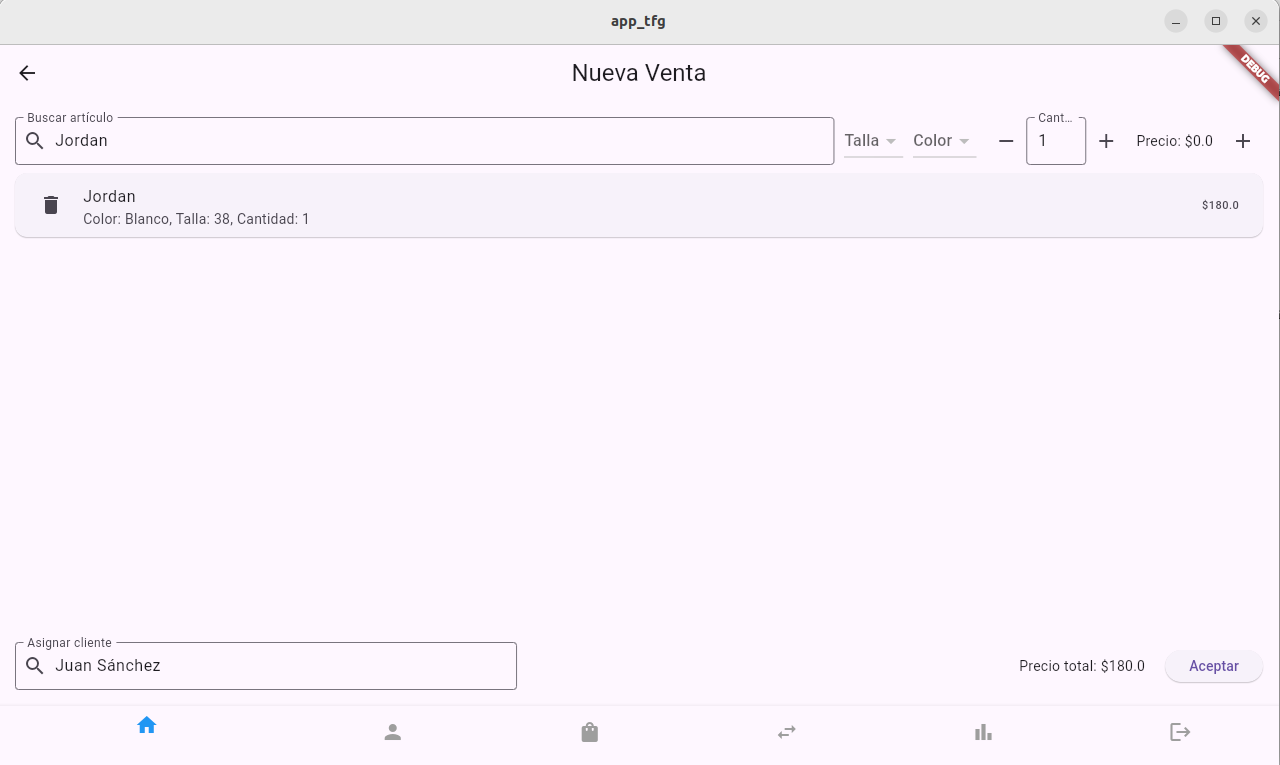
\includegraphics[width=0.7\textwidth]{imagenes/SegundaIteracion/nuevoPrestamo.png}
	\caption{Interfaz de usuario de la pantalla de nuevo préstamo.}
	\label{fig:appPantallaNuevoPrestamo}
\end{figure}

\subsubsection{Pantalla de visualización de movimientos}

En esta pantalla podemos ver todos los movimientos efectuados en la tienda. Están ordenados de forma que los más recientes se sitúen en la parte superior. Se puede eliminar un movimiento, pero se avisará de que el inventario no se actualizará. Esta funcionalidad es únicamente para permitir borrar movimientos que se generen por error. En la parte superior se puede buscar por cliente. Una vez seleccionado el cliente, solo aparecerán los movimientos que estén asociados a dicho cliente. Además, se puede filtrar por tipo de movimiento: Venta, Préstamo o Devolución. 

\begin{figure}[H]
	\centering
	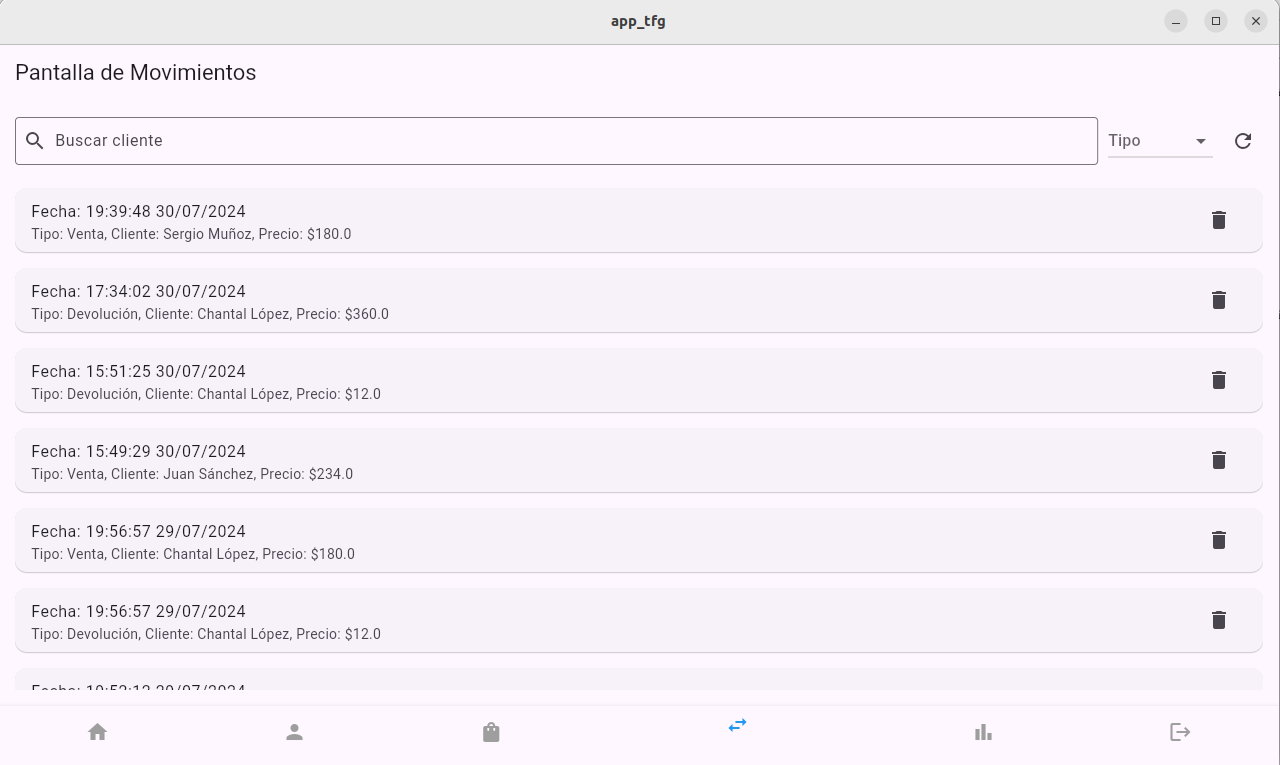
\includegraphics[width=0.7\textwidth]{imagenes/SegundaIteracion/listaMovimientos.png}
	\caption{Interfaz de usuario de la pantalla de visualización de movimientos.}
	\label{fig:appPantallaVisualizarMovimientos}
\end{figure}

\subsubsection{Pantalla de detalles del movimiento}

En esta pantalla podemos ver los detalles de un movimiento en específico. Esta pantalla muestra distintas funcionalidades dependiendo del tipo y del estado del movimiento. 

\textbf{Venta:} Cuando se trata de una venta, en la esquina superior derecha aparecen dos botones que te proponen una devolución parcial (solo quieres devolver algunos artículos) o una devolución total (se quieren devolver todos los artículos). Además, se pueden observar los datos relevantes de la venta, como los artículos involucrados, el cliente, el método de pago, la fecha y el precio total. 

\begin{figure}[H]
	\centering
	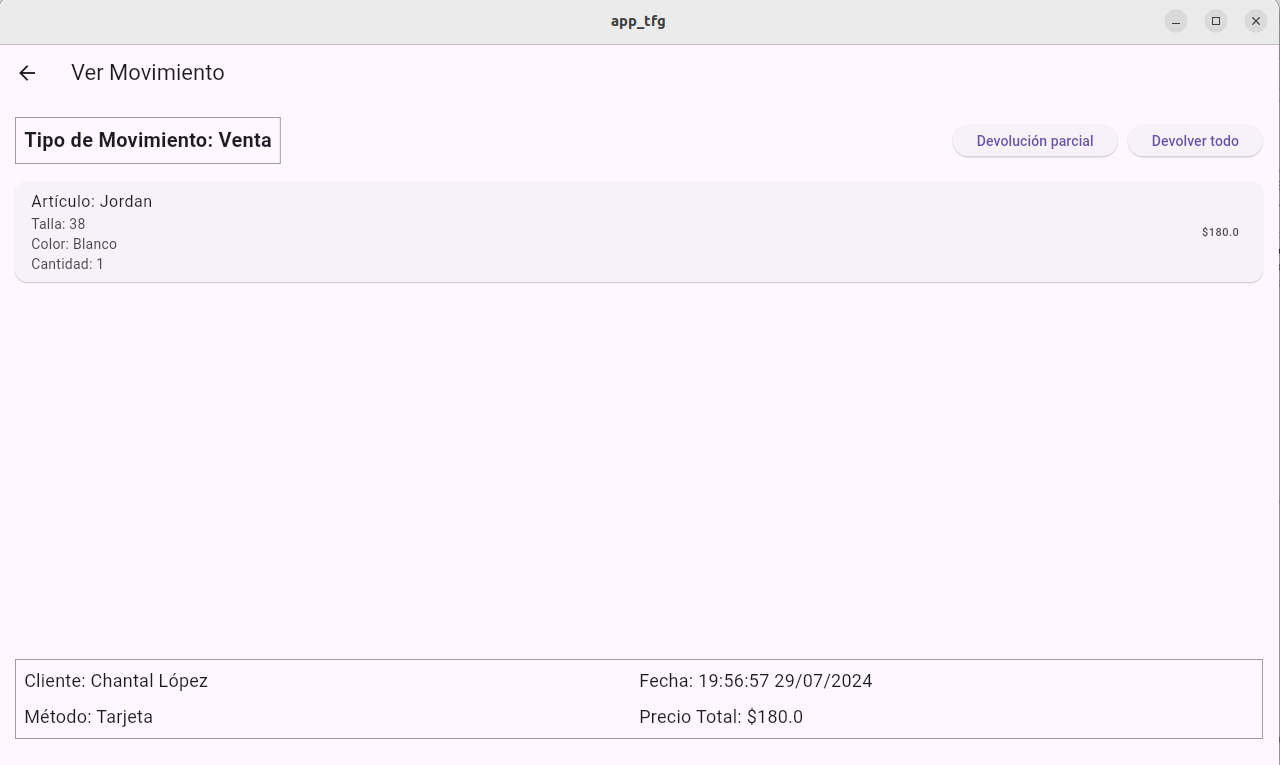
\includegraphics[width=0.7\textwidth]{imagenes/SegundaIteracion/detallesVenta.png}
	\caption{Interfaz de usuario de la pantalla de detalles de una venta.}
	\label{fig:appPantallaDetalleVenta}
\end{figure}

Si se realiza una devolución total, no se muestra ninguna pantalla adicional, directamente se crea un nuevo movimiento tipo Devolución con todos los artículos de la venta. Al realizar una devolución parcial, la pantalla cambia su modo Visualización a modo Devolución. Se permite escoger los artículos que se desean devolver y el método de pago en el que se prefiere realizar la devolución. 

\begin{figure}[H]
	\centering
	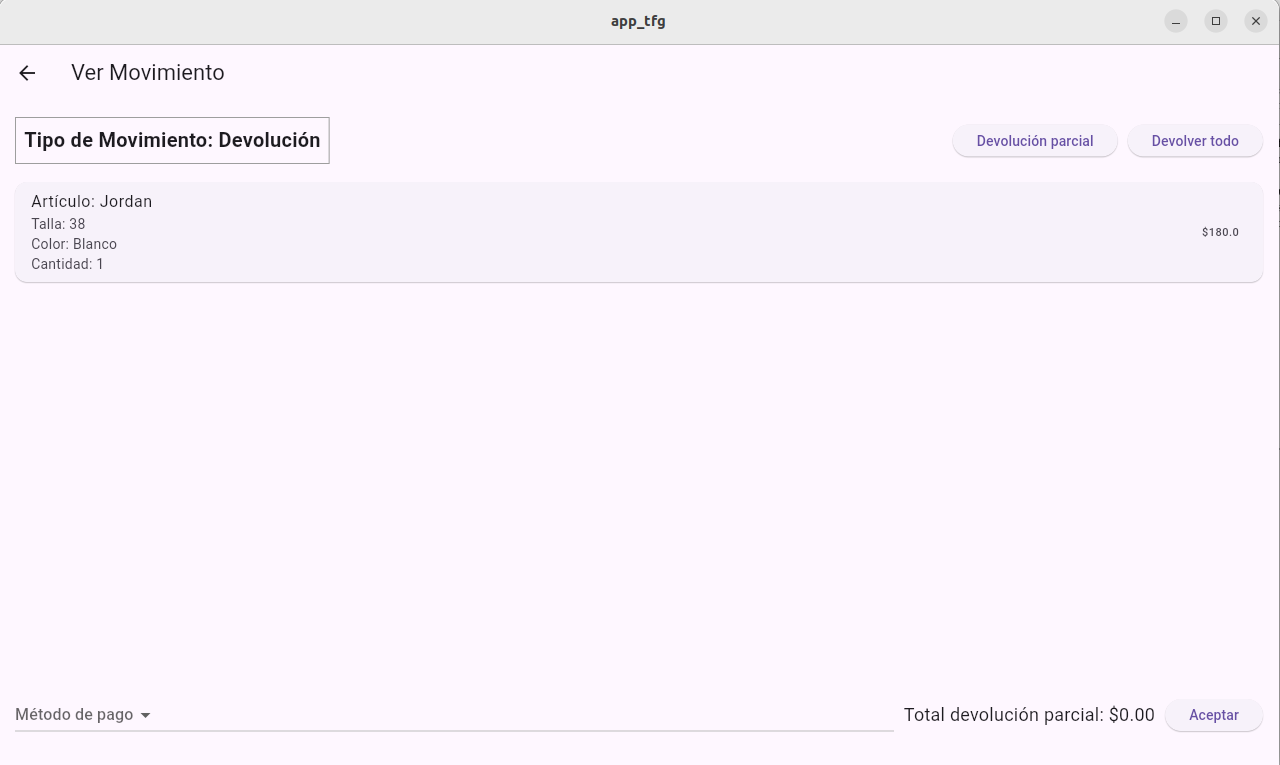
\includegraphics[width=0.7\textwidth]{imagenes/SegundaIteracion/devolucionVenta.png}
	\caption{Interfaz de usuario de la pantalla de devolución de una venta.}
	\label{fig:appPantallaDevolucionVenta}
\end{figure}

Tras aceptar la devolución, se genera un nuevo movimiento tipo Devolución. En la venta, se verá reflejada esta devolución. Desaparecen los botones de Devolución parcial y Devolución Total y aparece un botón con una referencia a la devolución realizada. De esta forma, se podrá visualizar de forma directa la devolución que se ha hecho de cada venta. 

\begin{figure}[H]
	\centering
	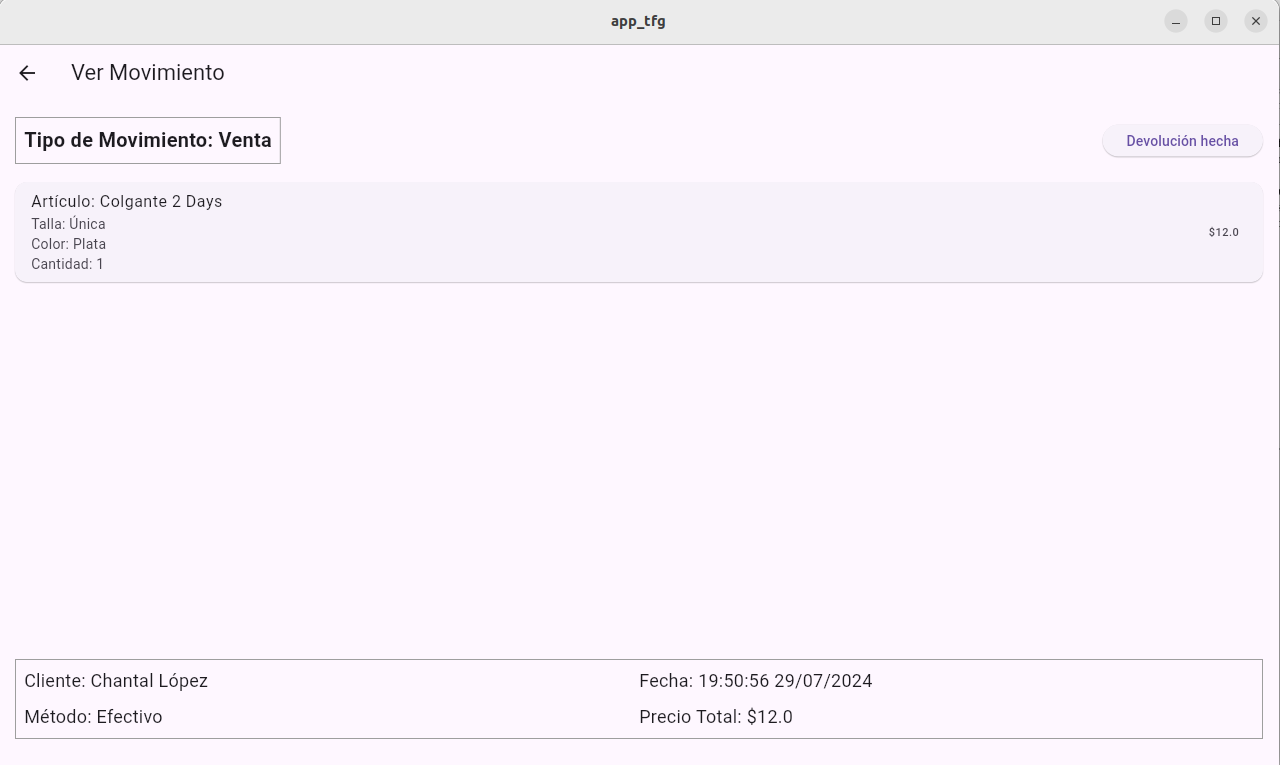
\includegraphics[width=0.7\textwidth]{imagenes/SegundaIteracion/devolucionHechaVenta.png}
	\caption{Interfaz de usuario de la pantalla de una venta con devolución hecha.}
	\label{fig:appPantallaDevolucionHechaVenta}
\end{figure}



\textbf{Pŕestamo: } La interfaz es similar a la pantalla de detalles de una venta, muestra la misma información. Sin embargo, los botones de la esquina superior son distintos. Una vez más, se ofrecen dos opciones: Compra o Devolver todo. El botón de Devolver todo funciona de la misma forma que en la Venta. 


\begin{figure}[H]
	\centering
	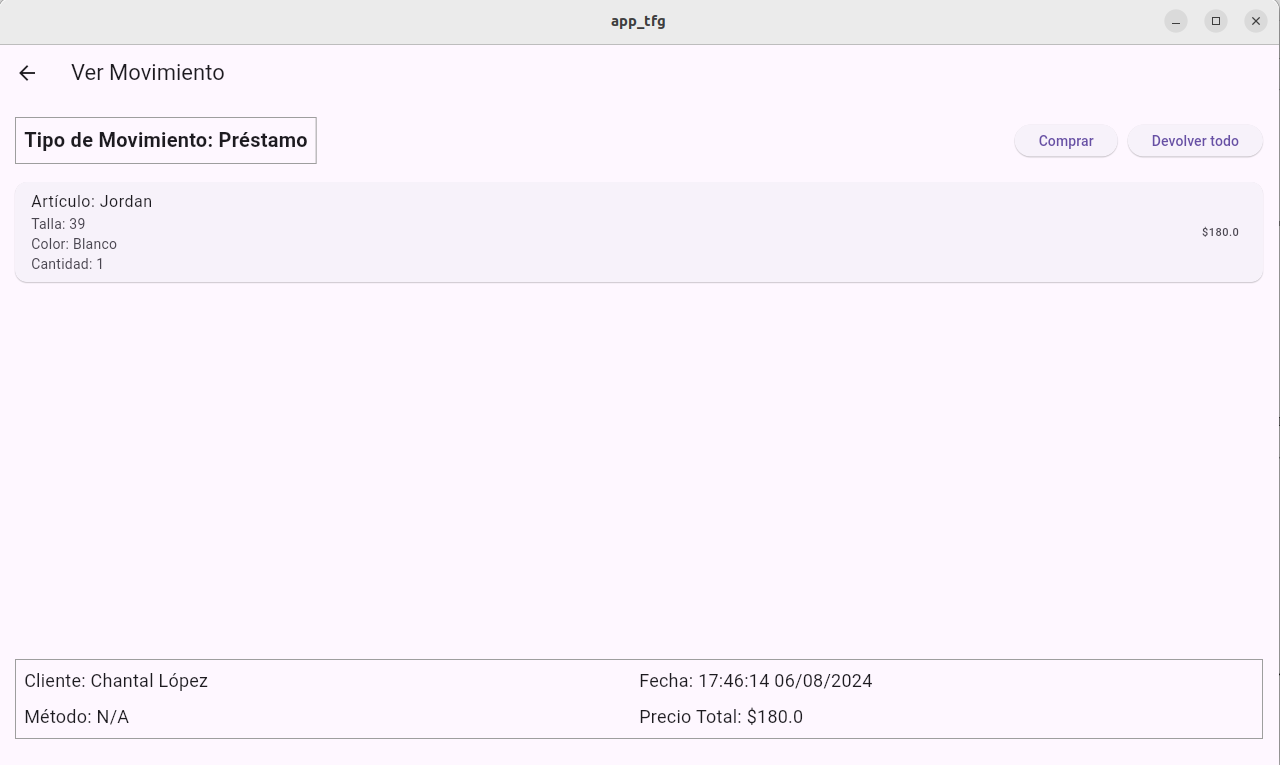
\includegraphics[width=0.7\textwidth]{imagenes/SegundaIteracion/detallesPrestamo.png}
	\caption{Interfaz de usuario de la pantalla los detalles de un préstamo.}
	\label{fig:appPantallaDetallesPrestamo}
\end{figure}

La funcionalidad del botón de Compra es distinta. Este botón permite generar una compra a partir de un préstamo. Al pulsar este botón, se cambia la funcionalidad de la pantalla y permite seleccionar los artículos que se desean comprar. Seleccionar el método de pago es obligatorio. Al seleccionar Aceptar, se generan dos movimientos: un movimiento de venta con los artículos que se han seleccionado para comprar y un movimiento de devolución con aquellos artículos que no se hayan comprado (en el caso de que queden artículos sin seleccionar). Así se verá reflejado en el historial de la tienda aquellos artículos que se compran y se devuelven. A su vez, el inventario se actualiza con estos movimientos. 

\begin{figure}[H]
	\centering
	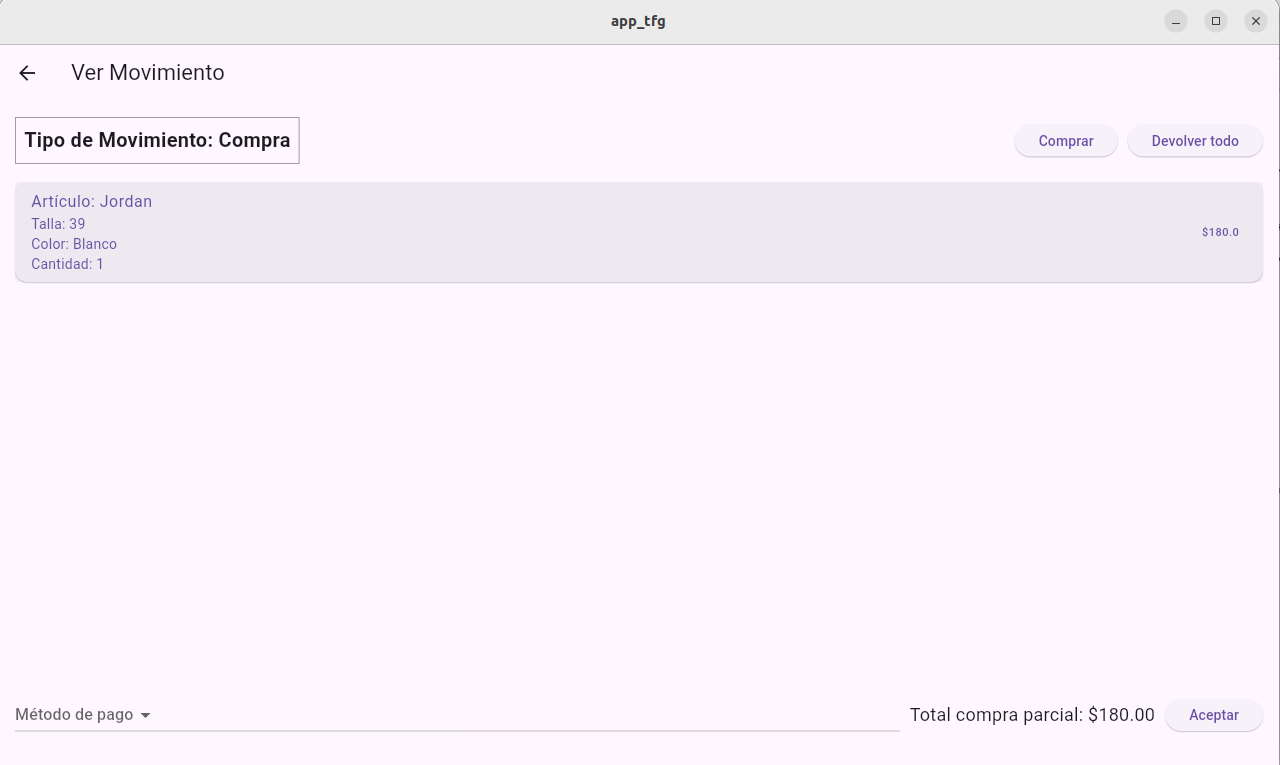
\includegraphics[width=0.7\textwidth]{imagenes/SegundaIteracion/compraPrestamo.png}
	\caption{Interfaz de usuario de la pantalla de compra a partir de un préstamo.}
	\label{fig:appPantallaCompraPrestamo}
\end{figure}

Si se ha hecho una devolución, se le asocia al préstamo de la misma forma que vimos en la venta.

\newpage

\textbf{Devolución: } Esta pantalla también muestra la misma información que los dos movimientos anteriores, los detalles del movimiento. En la esquina superior siempre aparecerá un botón de Movimiento original, que te llevará de forma directa al movimiento del cual proviene dicha devolución. 

\begin{figure}[H]
	\centering
	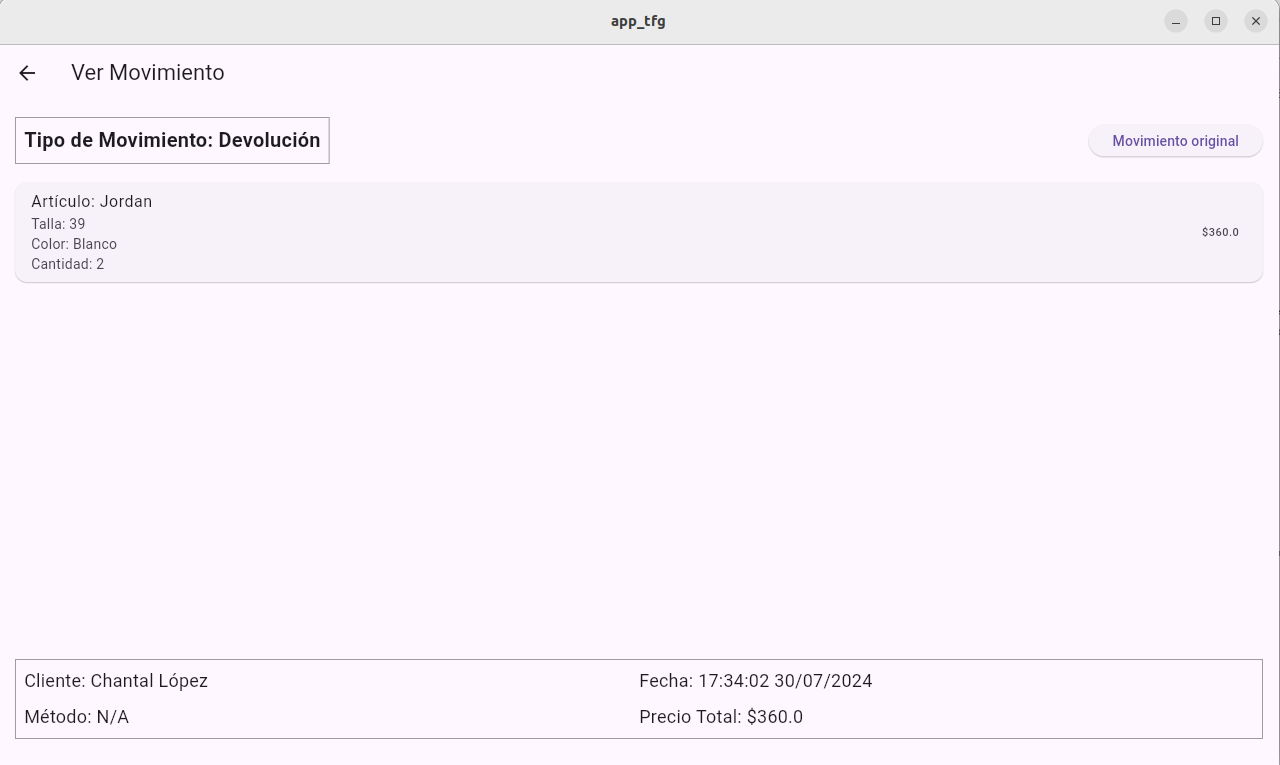
\includegraphics[width=0.7\textwidth]{imagenes/SegundaIteracion/detallesDevolucion.png}
	\caption{Interfaz de usuario de la pantalla de detalles de una devolución.}
	\label{fig:appPantallaDetallesDevolucion}
\end{figure}

\subsubsection{Mejora de las tallas en artículos}

En la iteración anterior, el cliente pidió que la gestión de las tallas de un artículo se hiciera de forma distinta. Se pidió que para cada artículo se pudieran añadir varias tallas. Para conseguir esto, se modifico la forma de crear un artículo, editarlo y visualizarlo. En la siguiente imagen podemos ver cómo la modificación ha sido correctamente efectuada. 

\begin{figure}[H]
	\centering
	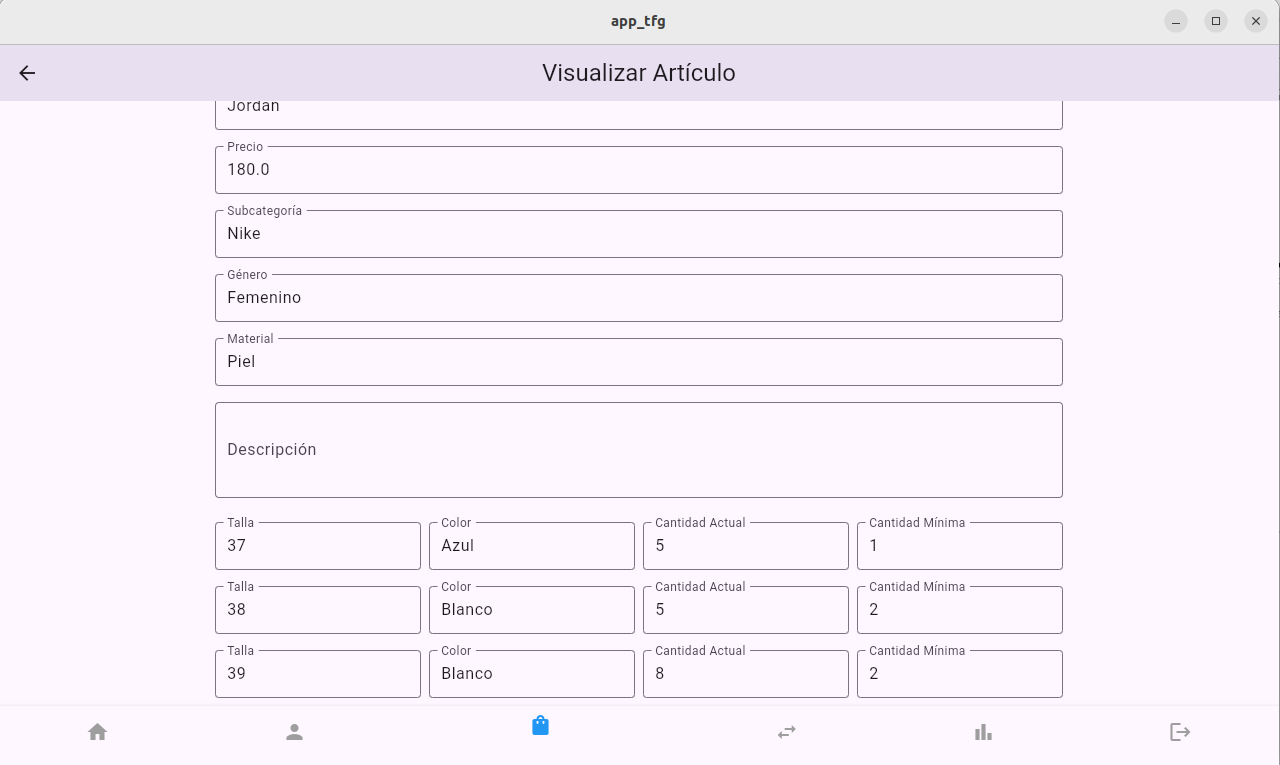
\includegraphics[width=0.7\textwidth]{imagenes/SegundaIteracion/tallasMultiples.png}
	\caption{Interfaz de usuario que muestra el cambio de la gestión de las tallas.}
	\label{fig:appPantallaDetallesDevolucion}
\end{figure}

\subsection{Revisión de la iteración}

El cliente probó el sistema ideado para los movimientos y expresó que estaba conforme con la lógica de la implementación. Además, mostró gratitud por el cambio de las tallas que solicitó en la iteración anterior. 

Por tanto, el cliente no puso ninguna objeción y animó a continuar con el planning establecido. 

\subsection{Plan para la próxima iteración}

Para la próxima iteración se propone: 

\begin{itemize}
	\item Implementar la pantalla de gráficos.
	\item Mejorar la interfaz gráfica, realizando a su vez, mejoras en la usabilidad y accesibilidad.
	\item Testeo de posibles fallos de funcionamiento de la aplicación.
\end{itemize}

\section{Tercera iteración}

\section{Creación y modificaciones de la base de datos}

\subsection{Creación de la base de datos}

Para crear la base de datos se ha utilizado la herramienta de Supabase. Esta herramienta permite crear una base de datos y sus tablas correspondientes de forma sencilla. Además, tiene una fácil integración con Flutter, por lo que conectar la aplicación a la base de datos no fue complicado. Fue suficiente con añadir librerías y las claves de configuración.  

Una vez configurada la base de datos dentro del proyecto, se genera una instancia que se utilizará cada vez que sea necesario hacer operaciones en la base de datos: 

\begin{figure}[H]
	\centering
	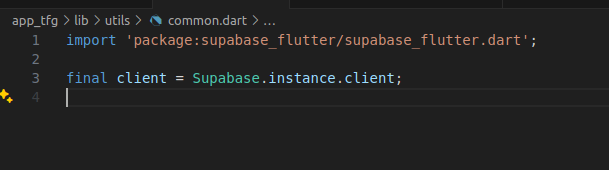
\includegraphics[width=0.7\textwidth]{imagenes/clientBD.png}
	\caption{Instancia de la base de datos.}
	\label{fig:instanciaBD}
\end{figure}

\subsection{Tablas de la base de datos}

Las tablas que están dentro de la base de datos son: 


\begin{itemize}
	\item \textbf{clientes:} En esta tabla se almacena toda la información relativa a los clientes. Podemos encontrar campos como el nombre, el teléfono, un comentario para añadir más información y una cartera, que permitirá que el cliente pueda tener dinero negativo o positivo en la tienda. 
	\item \textbf{categorias:} En esta tabla se crean categorías para organizar los artículos dentro de la tienda. Sus atributos tieneTamanio, tieneDescripcion, tieneMaterial, tieneGenero, son booleanos que permiten personalizar los atributos que tendrá un artículo. Si no se seleccionan alguno de estos atributos, todos los artículos que se creen bajo esa categoría no tendrán ese atributo. El atributo nombre indica el nombre de la categoría. 
	\item \textbf{articulos:} En esta tabla se almacena la información de cada uno de los artículos de la tienda. Sus atributos fijos son el nombre, el precio y la subcategoría (que permite categorizar más fino dentro de una categoría y posteriormente filtrar por dichas subcategorías). El resto de atributos son opcionales y se elegirán en la creación de la categoría de dicho artículo. Un artículo representa un modelo, dentro de una prenda podrán haber varias tallas o varios colores, lo que se contempla en la siguiente tabla. 
	\item \textbf{tallas:}  En esta tabla se registran las tallas y los colores disponibles de cada uno de los artículos. Para cada talla se especifica un color, la cantidad actual y la cantidad mínima. La cantidad mínima sirve para detectar cuando un artículo necesita ser renovado. Cuando se tienen igual o menos artículos de los especificados en la cantidad mínima, se mete en una lista de renovación de stock para indicar que deben ser renovados. 
	\item \textbf{movimientos:} En esta tabla se registra toda la información relacionada con los movimientos de la tienda. Se registra el precio total del movimiento, el cliente asignado, el método de pago, la fecha, el tipo de movimiento y el movimiento anterior, este atributo sirve para relacionar unos tickets con otros. Cuando se hace una devolución, se le asigna el movimiento anterior del que procede para poder ver cuál es su procedencia. Además, a las ventas / préstamos también se le asignan las devoluciones para una mejor sincronización.  
	\item \textbf{articulosMov:} En esta tabla se registran todos los artículos que pertenecen a cada movimiento. Es la tabla resultante de una relación muchos a muchos. Además, también se almacena como información adicional, la cantidad comprada de esa talla y el precio parcial. 
\end{itemize}


\subsection{Modificaciones intermedias de la base de datos}

Debido al cambio que solicitó el cliente con las tallas, se tuvo que crear una nueva tabla, la tabla tallas. Esto permitió que un artículo pudiera tener distintas tallas o distintos colores. 


\subsection{Diagrama final del diseño de la base de datos}

En este diagrama podemos ver los atributos que posee cada una de las tablas y como se relacionan entre ellas. Las líneas discontinuas indican las claves externas y los atributos con la llave a la izquierda representan las claves primarias de cada tabla. 

\begin{figure}[H]
	\centering
	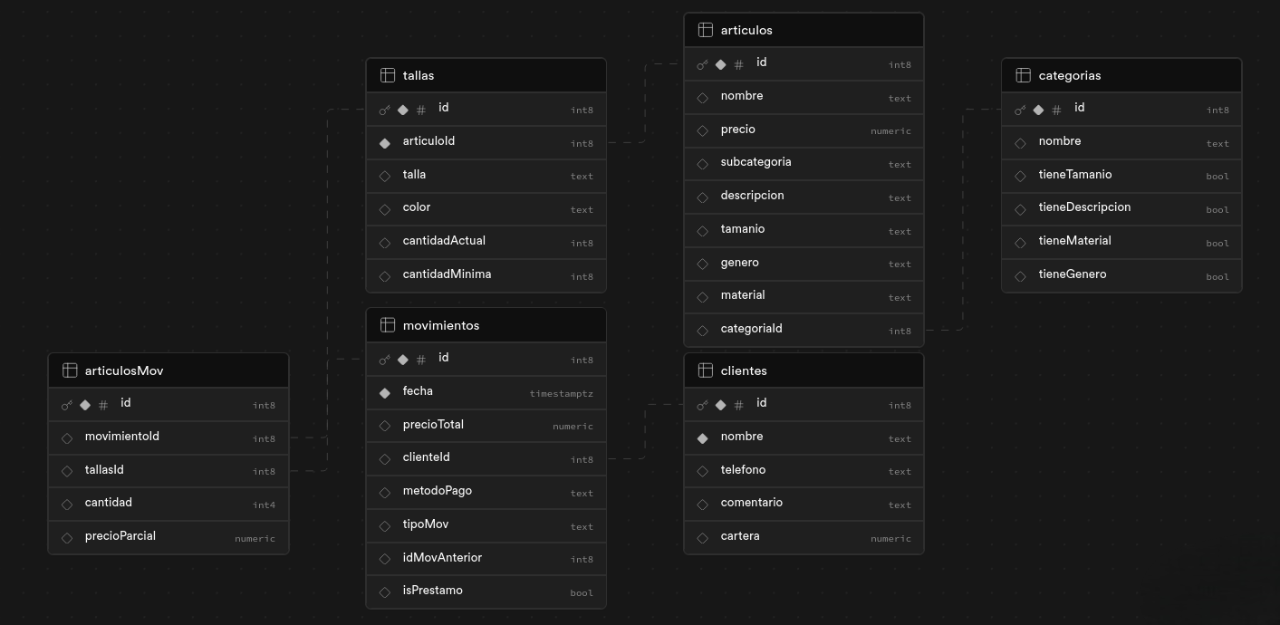
\includegraphics[width=0.7\textwidth]{imagenes/imagenesDiagramas/diagramaBD.png}
	\caption{Diagrama de la base de datos.}
	\label{fig:diagramaBD}
\end{figure}


